The first step in TRITIUM design was to choose the fiber length for a given fiber diameter ($1$ or $2~\mm$) at which the signal of tritium events is optimized. On the one hand, Long fibers are suitable because fewer fibers are needed to achieve the same TRITIUM detector efficiency as short fibers, reducing the price of the TRITIUM detector, but, on the other hand, in long fibers, scintillating photons are reflected on the fiber boundaries many times before reaching the photosensors, which may produce a deterioration in the tritium signal. To determine the optimal fiber length, several simulations, described in section \ref{subsec:FiberLengthSimulation}, were carried out using Geant4 \cite{Geant4WebPage}, a particle and nuclear physics simulation package based on C++. It was concluded that the optimal fiber length for the TRITIUM prototypes is around $20~\cm$, which is the fiber length used in TRITIUM prototypes developed at IFIC and it is also the length used for most of the experiments carried out in the framework of the TRITIUM experiment. As Saint-Gobain commercial fibers are longer than $20~\cm$, an effective scintillator cleaving technique had to be developed with strict requirements on the cleaving quality of the fiber ends since this greatly affects the transmission of photons and, consequently, the efficiency of TRITIUM monitor. This cleave must be done perpendicular to the fiber axis and with small uncertainty in the cleaving position to achieve a good end-surface quality that enables optimal coupling to the photosensor. It is also important that the fiber integrity be preserved, without cracks or deformations that contribute to the loss of photons. 

Cleaving the end faces of plastic polymer fibers is a current challenge. There are many different techniques such as milling, laser cleaving, focused-ion-beam, blade cleaving, etc. The blade cleaving technique was chosen for TRITIUM experiment because of its mechanical simplicity and because this preserve the integrity of plastice fibers. Many commercial devices based on blade cleaving, such as the one provided by Thorlabs with a diamond tipped blade \cite{DiamondThorlabs} or others similar to guillotine designed for industrial fiber optics \cite{GuillotineIFO}, were tested in an extensive study with unsuccessful results \cite{TFGAlberto}. As it can be seen in Figures \ref{fig:BadCleavesOfFibers}, commercial techniques produce deformations, cracks and imperfections so they do not fulfill the quality standard requirements for the detector.

\begin{figure}
\centering
    \begin{subfigure}[b]{0.5\textwidth}
    \centering
    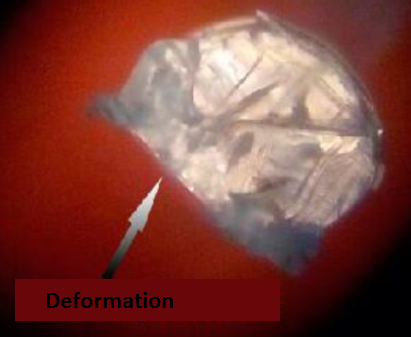
\includegraphics[width=\textwidth]{4ResearchAndDevelopments/41Fibers/DeformationFiberEnds.png}  
    \caption{\label{subfig:FiberEndDeformation}}
    \end{subfigure}
    \hfill
    \begin{subfigure}[b]{0.45\textwidth}
    \centering
    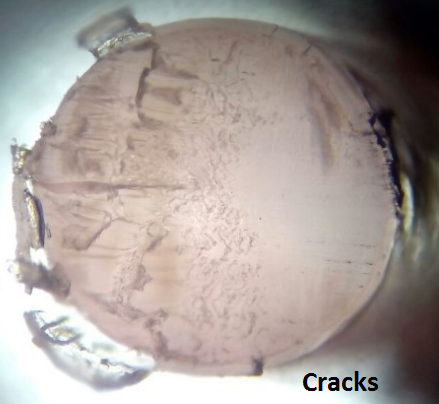
\includegraphics[width=\textwidth]{4ResearchAndDevelopments/41Fibers/CracksEndFibers.png}  
    \caption{\label{subfig:FiberEndCracks}}
    \end{subfigure}
 \caption{Unsuccessful results of using commercial techniques for cleaving the scintillating fibers a) Fiber end deformation b) Fiber end cracks. Pictures taken with the microscope PB 4161 from EUROMEX.}
 \label{fig:BadCleavesOfFibers}
\end{figure}

Because commercial devices are not suitable for polymer fibers, a cleaving device, shown in Figure \ref{fig:CleaveTRITIUMDevice}, was designed, built and tested at IFIC laoratory.

\begin{figure}
\centering
    \begin{subfigure}[b]{0.5\textwidth}
    \centering
    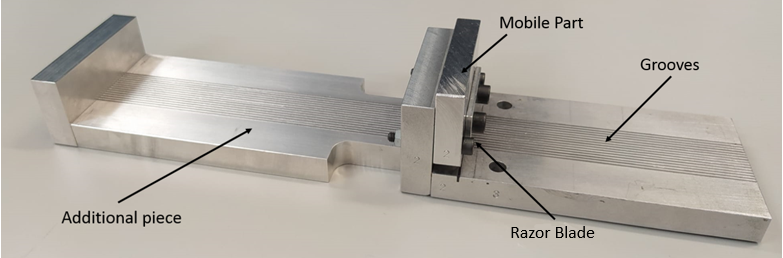
\includegraphics[width=\textwidth]{4ResearchAndDevelopments/41Fibers/CuttingDevice.png}  
    \caption{\label{subfig:CleaveTRITIUMDevice1}}
    \end{subfigure}
    \hfill
    \begin{subfigure}[b]{0.45\textwidth}
    \centering
    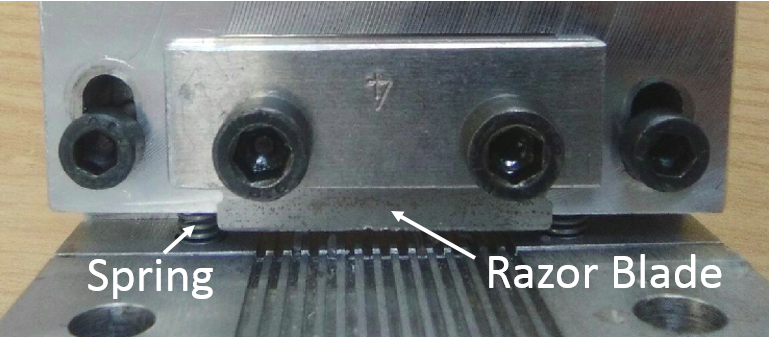
\includegraphics[width=\textwidth]{4ResearchAndDevelopments/41Fibers/Cleaving_machine_ZOOM.png}  
    \caption{\label{subfig:CleaveTRITIUMDeviceZOOM}}
    \end{subfigure}
 \caption{Cleaving device developed in TRITIUM experiment. \label{fig:CleaveTRITIUMDevice}}
\end{figure}

%\begin{figure}[hbtp]
%\centering
%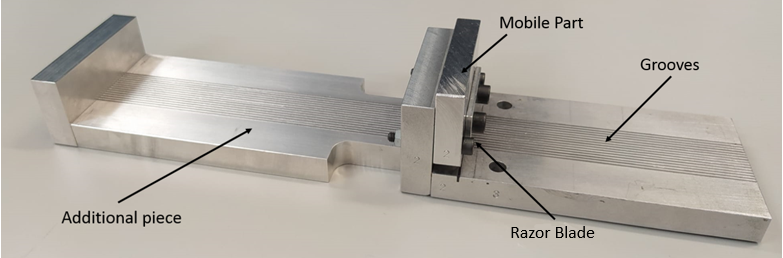
\includegraphics[scale=0.4]{4ResearchAndDevelopments/41Fibers/CuttingDevice.png}
%\caption{Cleaving device developed in TRITIUM experiment. \label{fig:CleaveTRITIUMDevice}}
%\end{figure}

This device consists of fourteen grooves used for lodging the fibers and a thin razor blade, attached to a mobile piece, which is used to cleave them. The perpendicular cleave, which is one of the requirements, can be ensured since the moving piece to which the blade is attached, is set perpendicular to the fibers. The blade used is a typical commercial razor blade, of $0.1~\mm$ thickness, which is the thickness that gave the best results. The blade was positioned with a $5\degree$ inclination with respect to the horizontal axis since it was found in several studies that this helps to obtain a less aggressive and cleaner cleave \cite{AngleBlade, TemperatureBlade}. As it can be seen in Figure \ref{fig:CleavingFiberEnd}, with this cleaving device fiber ends without breaks or deformation were obtained. An additional parameter that could affect the cleaving quality of the fiber ends is the temperature of both fiber and blade. A study was carried out in which both were subject to different temperatures from room temperature to 110 degrees. No significant conclusions were obtained \cite{TFGAlberto}. Thus, the cleaving process was carried out at room temperature to make the cleaving process easier.

\begin{figure}[h]
\centering
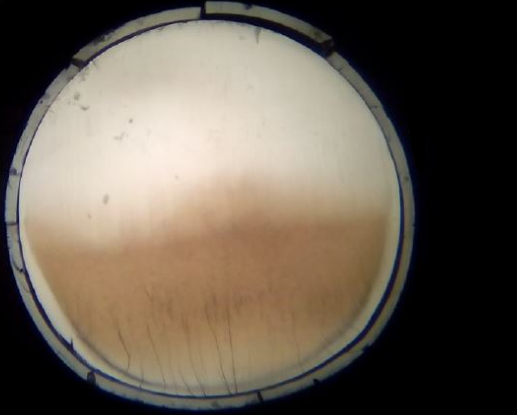
\includegraphics[scale=0.75]{4ResearchAndDevelopments/41Fibers/CutEndFiberGood.png}
\caption{Fiber end after cleaving process using the cleaving machine developed. Pictures taken with the microscope PB 4161 from EUROMEX.\label{fig:CleavingFiberEnd}}
\end{figure}

Finally, to set the fiber length an additional piece was designed and built, shown in Figure \ref{fig:CleaveTRITIUMDevice}, with which a length uncertainty of less than 1 millimeter in the fiber length was achieved.